\chapter{Specifikacija programske potpore}
		
	\section{Funkcionalni zahtjevi}
			
			%\textbf{\textit{dio 1. revizije}}\\
			
%			\textit{Navesti \textbf{dionike} koji imaju \textbf{interes u ovom sustavu} ili  \textbf{su nositelji odgovornosti}. To su prije svega korisnici, ali i administratori sustava, naručitelji, razvojni tim.}\\
%				
%			\textit{Navesti \textbf{aktore} koji izravno \textbf{koriste} ili \textbf{komuniciraju sa sustavom}. Oni mogu imati inicijatorsku ulogu, tj. započinju određene procese u sustavu ili samo sudioničku ulogu, tj. obavljaju određeni posao. Za svakog aktora navesti funkcionalne zahtjeve koji se na njega odnose.}\\
			
			
			\noindent \textbf{Dionici:}
			
			\begin{packed_enum}
				
				\item Korisnici (učenici)
				\item Administrator riječi				
				\item Razvojni tim
				\item Konkurencija
				\item Naručitelj
				
			\end{packed_enum}
			
			\noindent \textbf{Aktori i njihovi funkcionalni zahtjevi:}
			
			
			\begin{packed_enum}
				\item  \underbar{Učenik može:}
				
				\begin{packed_enum}
					
					\item registrirati se
					\item prijaviti se
					\item odjaviti se
%					\begin{packed_enum}
%						
%						\item  podfunkcionalnost 1 
%						\item  podfunkcionalnost 2
%				
%					\end{packed_enum}
					\item odabrati rječnik i mod učenja
					\item odgovarati na pitanja
					\item obrisati svoj korisnički račun
					\item izmijeniti osobne podatke svog korisničkog računa
					
				\end{packed_enum}
			
				\item  \underbar{Administrator riječi može:}
				
				\begin{packed_enum}
					
					\item dodati riječ u rječnik
					\item urediti komponente riječi
					\item ukloniti riječ iz baze
					\item kreirati novi rječnik
					\item obrisati rječnik
					\item dodati novog administratora
					\item obrisati postojećeg korisnika
					\item izmijeniti osobne podatke postojećeg korisnika
										
				\end{packed_enum}
				
				\item  \underbar{Baza podataka može:}
				
				\begin{packed_enum}
					
					\item pohranjivati podatke o korisnicima (učenici i administratori riječi)
					\item pohranjivati podatke o dostupnim jezicima, rječnicima i riječima
					\item za svakog korisnika pohranjivati zadnje stanje učenja i posude riječi
					
				\end{packed_enum}
				
				\item  \underbar{Vanjski rječnik može:}
				
				\begin{packed_enum}
					
					\item dohvatiti riječi na temelju upisanog predloška (dijela riječi)
					
				\end{packed_enum}
				
				\item  \underbar{Servis za ocjenu izgovora može:}
				
				\begin{packed_enum}
					
					\item ocijeniti kvalitetu izgovorene riječi na temelju predane zvučne datoteke
					
				\end{packed_enum}
				
			\end{packed_enum}
			
			\eject 
			
			
				
			\subsection{Obrasci uporabe}
				
% {dio 1. revizije}}
				
				\subsubsection{Opis obrazaca uporabe}
%{Funkcionalne zahtjeve razraditi u obliku obrazaca uporabe. Svaki obrazac je potrebno razraditi prema donjem predlošku. Ukoliko u nekom koraku može doći do odstupanja, potrebno je to odstupanje opisati i po mogućnosti ponuditi rješenje kojim bi se tijek obrasca vratio na osnovni tijek.}
					


					\noindent \underbar{\textbf{UC1 - Registracija}}
					\begin{packed_item}
	
						\item \textbf{Glavni sudionik: }Učenik
						\item  \textbf{Cilj:} Kreiranje novog korisničkog računa kojim se omogućuje pristup sustavu
						\item  \textbf{Sudionici:} Baza podataka
						\item  \textbf{Preduvjet:} -
						\item  \textbf{Opis osnovnog tijeka:}  
						
						\item[] \begin{packed_enum}
	
							\item Korisnik odabire opciju registracije
							\item Sustav prikazuje formu za unos podataka (ime, prezime, elektronička pošta, zaporka)
							\item Korisnik unosi podatke i potvrđuje registraciju
							\item Sustav pohranjuje podatke i novom korisniku šalje elektroničku poštu s inicijalnom lozinkom
							
						\end{packed_enum}
						
						\item  \textbf{Opis mogućih odstupanja:}
						
						\item[] \begin{packed_item}
	
							\item[3.a] Korisnik odustaje od registracije
							\item[] \begin{packed_enum}
								
								\item Sustav se vraća na početnu stranicu
								
							\end{packed_enum}
							
							\item[3.b] Nevažeća adresa elektroničke pošte
							\item[] \begin{packed_enum}
								
								\item Sustav obavještava korisnika kako je nepravilno unesena adresa elektroničke pošte te prikazuje važeći oblik adrese elektroničke pošte
								
							\end{packed_enum}
							
							\item[4.a] U sustavu već postoji korisnik s istom adresom elektroničke pošte
							\item[] \begin{packed_enum}
								
								\item Sustav obavještava korisnika da se adresa elektroničke pošte već koristi
								
								\item Sustav ponovno prikazuje formu za unos podataka
								
							\end{packed_enum}
							

						\end{packed_item}
					\end{packed_item}
					
					
					\noindent \underbar{\textbf{UC2 - Prijava}}
					\begin{packed_item}
						
						\item \textbf{Glavni sudionik: }Učenik, administrator riječi
						\item  \textbf{Cilj:} Pristupiti sustavu učenja
						\item  \textbf{Sudionici:} Baza podataka
						\item  \textbf{Preduvjet:} UC1 (Registracija) za učenika
						\item  \textbf{Opis osnovnog tijeka:}
						
						\item[] \begin{packed_enum}
							
							\item Korisnik odabire opciju prijava
							\item Sustav prikazuje formu za unos podataka
							\item Korisnik unosi podatke i potvrđuje prijavu
							\item Sustav otvara stranicu s ponuđenim jezicima
						\end{packed_enum}
						
						\item  \textbf{Opis mogućih odstupanja:}
						
						\item[] \begin{packed_item}
							
							\item[3.a] Korisnik odustaje od prijave
							\item[] \begin{packed_enum}
								
								\item Sustav prikazuje početnu stranicu
								
							\end{packed_enum}
							
							\item[3.b] Uneseni podatci za prijavu su netočni
							\item[] \begin{packed_enum}
								
								\item Sustav obavještava korisnika da su uneseni podatci netočni te i dalje prikazuje formu za unos podataka
								
							\end{packed_enum}
							
							\item[3.c] Korisnik se prijavljuje po prvi put
							\item[] \begin{packed_enum}
								
								\item Sustav prikazuje formu za promjenu zaporke
								
							\end{packed_enum}
							
							
						\end{packed_item}
					\end{packed_item}
					
						\noindent \underbar{\textbf{UC3 - Odjava}}
					\begin{packed_item}
						
						\item \textbf{Glavni sudionik: }Učenik, administrator riječi
						\item  \textbf{Cilj:} Omogućiti napuštanje sustava učenja
						\item  \textbf{Sudionici:} Baza podataka
						\item  \textbf{Preduvjet:} UC2 (Prijava)
						\item  \textbf{Opis osnovnog tijeka:}
						
						\item[] \begin{packed_enum}
							
							\item Korisnik odabire opciju "Odjava"
							\item Sustav prikazuje početnu stranicu
						\end{packed_enum}
					\end{packed_item}
					
						\noindent \underbar{\textbf{UC4 - Odabir jezika}}
					\begin{packed_item}
						
						\item \textbf{Glavni sudionik: }Učenik, administrator riječi
						\item  \textbf{Cilj:} Pristup dostupnim rječnicima za neki od jezika ponuđenih u sustavu
						\item  \textbf{Sudionici:} Baza podataka
						\item  \textbf{Preduvjet:} UC2 (Prijava)
						\item  \textbf{Opis osnovnog tijeka:}
						
						\item[] \begin{packed_enum}
							
							\item Korisnik odabire jezik
							\item Sustav prikazuje stranicu s odabirom rječnika
						\end{packed_enum}
						
						\item  \textbf{Opis mogućih odstupanja:}
						
						\item[] \begin{packed_item}
							
							\item[1.a] Korisnik pristupa jeziku koji nije podržan
							\item[] \begin{packed_enum}
								
								\item Sustav obavještava korisnika kako odabrani jezik nije podržan
								\item Sustav prikazuje stranicu s ponuđenim jezicima
								
							\end{packed_enum}
							
						\end{packed_item}
						
					\end{packed_item}
					
					
					\noindent \underbar{\textbf{UC5 - Odabir rječnika}}
					\begin{packed_item}
						
						\item \textbf{Glavni sudionik: }Učenik, administrator riječi
						\item  \textbf{Cilj:} Pristup nekom od dostupnih rječnika za prije odabrani jezik
						\item  \textbf{Sudionici:} Baza podataka
						\item  \textbf{Preduvjet:} UC4 (Odabir jezika)
						\item  \textbf{Opis osnovnog tijeka:}
						
						\item[] \begin{packed_enum}
							
							\item Korisnik odabire rječnik
							\item Sustav prikazuje stranicu za odabrani rječnik
						\end{packed_enum}
						
						\item  \textbf{Opis mogućih odstupanja:}
						
						\item[] \begin{packed_item}
							
							\item[1.a] Korisnik odabire rječnik koji ne postoji u sustavu
							\item[] \begin{packed_enum}
								
								\item Sustav obavještava korisnika kako se odabrani rječnik ne nalazi u sustavu
								\item Sustav prikazuje stranicu za odabir rječnika
								
							\end{packed_enum}
							
							\item[1.b] Za ponuđeni rječnik, ne postoje dostupne riječi za korisnika
							\item[] \begin{packed_enum}
								
								\item Sustav obavještava korisnika kako je potrebno vratiti se kasnije za učenje riječi iz odabranog rječnika
								\item Sustav otvara prikaz dostupnih rječnika za odabrani jezik
								
							\end{packed_enum}
							
							\item[1.c] Učenik je naučio sve riječi iz odabranog rječnika
							\item[] \begin{packed_enum}
								
								\item Sustav obavještava korisnika kako je naučio sve riječi iz rječnika
								\item Sustav otvara prikaz dostupnih rječnika za odabrani jezik
								
							\end{packed_enum}
							
						\end{packed_item}
					\end{packed_item}
					
					\noindent \underbar{\textbf{UC6 - Odabir moda učenja}}
					\begin{packed_item}
						
						\item \textbf{Glavni sudionik: }Učenik
						\item  \textbf{Cilj:} Odabir jednog od ponuđenih modova učenja 
						\item  \textbf{Sudionici:} Baza podataka
						\item  \textbf{Preduvjet:} UC5 (Odabir rječnika)
						\item  \textbf{Opis osnovnog tijeka:}
						
						\item[] \begin{packed_enum}
							
							\item Sustav prikazuje sve ponuđene modove učenja za odabrani rječnik (upit engleske riječi uz odabir hrvatskog prijevoda, upit hrvatske riječi uz odabir engleskog prijevoda, upit izgovorom engleske riječi uz odgovor pisanjem riječi na engleskom, upit tekstualnim oblikom engleske riječi uz snimanje izgovora u glasovnu datoteku)
							\item Učenik odabire jedan od ponuđenih modova
							\item Sustav okreće kviz
							\item Sustav prikazuje prvo pitanje
							
						\end{packed_enum}
						
						\item  \textbf{Opis mogućih odstupanja:}
						
						\item[] \begin{packed_item}
							
							\item[2.a] Učenik odabire mod koji nije podržan 
							\item[] \begin{packed_enum}
								
								\item Sustav ponovno otvara stranicu s prikazom ponuđenih modova
								
							\end{packed_enum}
							
						\end{packed_item}
							
					\end{packed_item}
					
					\noindent \underbar{\textbf{UC7 - Odgovor na pitanje}}
					\begin{packed_item}
						
						\item \textbf{Glavni sudionik: } Učenik
						\item  \textbf{Cilj:} Dobiti odgovor na postavljeno pitanje od korisnika
						\item  \textbf{Sudionici:} Baza podataka
						\item  \textbf{Preduvjet:} UC6 (Odabir moda učenja)
						\item  \textbf{Opis osnovnog tijeka:}
						
						\item[] \begin{packed_enum}
							
							\item Korisnik daje odgovor
							\item Sustav pohranjuje odgovor i obavještava korisnika o točnosti njegovog odgovora
							\item Korisnik odabire opciju "Nastavi"
							\item Sustav prikazuje sljedeće pitanje
						\end{packed_enum}
						
						\item  \textbf{Opis mogućih odstupanja:}
						
						\item[] \begin{packed_item}
							
							\item[3.a] Korisnik odustaje od kviza
							\item[] \begin{packed_enum}
								
								\item Sustav prikazuje stranicu s odabirom rječnika
								
							\end{packed_enum}
							
							\item[4.a] Korisnik odustaje od kviza 
							\item[] \begin{packed_enum}
								
								\item Sustav prikazuje stranicu s odabirom rječnika
								
							\end{packed_enum}
							
						\end{packed_item}
					\end{packed_item}
					
					\noindent \underbar{\textbf{UC7.1 - Odabir odgovora}}
					\begin{packed_item}
						
						\item \textbf{Glavni sudionik: }Učenik
						\item  \textbf{Cilj:} Dobiti odgovor od učenika tako što učenik odabire jedan od ponuđenih odgovora 
						\item  \textbf{Sudionici:} Baza podataka
						\item  \textbf{Preduvjet:} UC6 (Odabir moda učenja)
						\item  \textbf{Opis osnovnog tijeka:}
						
						\item[] \begin{packed_enum}
							
							\item Korisnik odabire jedan odgovor među ponuđenima
							\item Sustav pohranjuje odgovor i obavještava korisnika o točnosti njegovog odgovora
							\item Korisnik odabire opciju "Nastavi"
							\item Sustav prikazuje sljedeće pitanje
						\end{packed_enum}
						
						\item  \textbf{Opis mogućih odstupanja:}
						
						\item[] \begin{packed_item}
							
							\item[3.a] Korisnik odustaje od kviza
							\item[] \begin{packed_enum}
								
								\item Sustav prikazuje stranicu s odabirom rječnika
								
							\end{packed_enum}
							
							\item[4.a] Korisnik odustaje od kviza 
							\item[] \begin{packed_enum}
								
								\item Sustav prikazuje stranicu s odabirom rječnika
								
							\end{packed_enum}
							
						\end{packed_item}
					\end{packed_item}
					
					\noindent \underbar{\textbf{UC7.2 - Unos odgovora}}
					\begin{packed_item}
						
						\item \textbf{Glavni sudionik: }Učenik
						\item  \textbf{Cilj:} Dobiti od učenika odgovor na pitanje tako što učenik upisuje odgovor
						\item  \textbf{Sudionici:} Baza podataka
						\item  \textbf{Preduvjet:} UC6 (Odabir moda učenja)
						\item  \textbf{Opis osnovnog tijeka:}
						
						\item[] \begin{packed_enum}
							
							\item Korisnik unosi odgovor u polje za unos odgovora i potvrđuje klikom na gumb
							\item Sustav pohranjuje odgovor i obavještava korisnika o točnosti njegovog odgovora
							\item Korisnik odabire opciju "Nastavi"
							\item Sustav prikazuje sljedeće pitanje
						\end{packed_enum}
						
						\item  \textbf{Opis mogućih odstupanja:}
						
						\item[] \begin{packed_item}
							
							\item[1.a] Korisnik unosi odgovor u neispravnom formatu 
							\item[] \begin{packed_enum}
								
								\item Sustav obavještava učenika kako se u odgovoru koriste nepodržani znakovi
								\item Sustav ponovno prikazuje pitanje
								
							\end{packed_enum}
								
							
							\item[3.a] Korisnik odustaje od kviza
							\item[] \begin{packed_enum}
								
								\item Sustav prikazuje stranicu s odabirom rječnika
								
							\end{packed_enum}
							
							\item[4.a] Korisnik odustaje od kviza 
							\item[] \begin{packed_enum}
								
								\item Sustav prikazuje stranicu s odabirom rječnika
								
							\end{packed_enum}
							
						\end{packed_item}
					\end{packed_item}
					
					\noindent \underbar{\textbf{UC7.3 - Snimanje izgovora u zvučnu datoteku}}
					\begin{packed_item}
						
						\item \textbf{Glavni sudionik: }Učenik
						\item  \textbf{Cilj:} Dobiti odgovor od učenika tako što učenik snima zvučni zapis
						\item  \textbf{Sudionici:} Baza podataka, servis za ocjenu izgovora
						\item  \textbf{Preduvjet:} UC6 (Odabir moda učenja)
						\item  \textbf{Opis osnovnog tijeka:}
						
						\item[] \begin{packed_enum}
							
							\item Korisnik snima izgovor u zvučnu datoteku
							\item Sustav pohranjuje zvučnu datoteku i pokreće ocjenu kvalitete izgovorene riječi
							\item Sustav obavještava korisnika o točnosti njegovog odgovora
							\item Korisnik odabire opciju "Nastavi"
							\item Sustav prikazuje sljedeće pitanje
						\end{packed_enum}
						
						\item  \textbf{Opis mogućih odstupanja:}
						
						\item[] \begin{packed_item}
							
								
							\item[2.a] Neuspješno pohranjivanje zvučne datoteke 
							\item[] \begin{packed_enum}
								
								\item Sustav ponovno prikazuje pitanje
								\item Sustav od učenika traži ponovni unos odgovora snimanjem
								
							\end{packed_enum}
								
							\item[2.b] Neuspješno pokretanje ocjene kvalitete izgovora 
							\item[] \begin{packed_enum}
								
								\item Sustav od učenika traži ponovni pokušaj pohrane rješenja
								
							\end{packed_enum}
							
							\item[3.a] Korisnik odustaje od kviza
							\item[] \begin{packed_enum}
								
								\item Sustav prikazuje stranicu s odabirom rječnika
								
							\end{packed_enum}
							
							\item[4.a] Korisnik odustaje od kviza 
							\item[] \begin{packed_enum}
								
								\item Sustav prikazuje stranicu s odabirom rječnika
								
							\end{packed_enum}
							
						\end{packed_item}
					\end{packed_item}
					
					\noindent \underbar{\textbf{UC8 - Brisanje korisničkog računa}}
					\begin{packed_item}
						
						\item \textbf{Glavni sudionik: }Učenik
						\item  \textbf{Cilj:} Uklanjanje korisničkog računa iz sustava
						\item  \textbf{Sudionici:} Baza podataka
						\item  \textbf{Preduvjet:} UC2 (Prijava)
						\item  \textbf{Opis osnovnog tijeka:}
						
						\item[] \begin{packed_enum}
							
							\item Korisnik odabire opciju brisanja korisničkog računa
							\item Sustav prikazuje prozor s upitom "Jeste li sigurni da želite obrisati svoj korisnički račun?"
							\item Korisnik odabire opciju "Da"
							\item Sustav briše korisnički račun i prikazuje početnu stranicu
						\end{packed_enum}
						
						\item  \textbf{Opis mogućih odstupanja:}
						
						\item[] \begin{packed_item}
							
							\item[3.a] Korisnik odabire opciju "Ne"
							\item[] \begin{packed_enum}
								
								\item Sustav zatvara prozor
								\item Sustav prikazuje stranicu s odabirom jezika
								
							\end{packed_enum}
							
						\end{packed_item}
					\end{packed_item}
					
					\noindent \underbar{\textbf{UC9 - Kreiranje novog rječnika}}
					\begin{packed_item}
						
						\item \textbf{Glavni sudionik: }Administrator riječi
						\item  \textbf{Cilj:} Kreiranje novog rječnika
						\item  \textbf{Sudionici:} Baza podataka
						\item  \textbf{Preduvjet:} UC18 (Dodavanje jezika)
						\item  \textbf{Opis osnovnog tijeka:}
						
						\item[] \begin{packed_enum}
							
							\item Administrator riječi odabire opciju "Kreiraj novi rječnik"
							\item Sustav otvara formu za upis podataka o rječniku 
							\item Administrator riječi upisuje sve potrebne podatke
							\item Administrator riječi odabire opciju "Spremi"
							\item Sustav sprema promjene i prikazuje početnu stranicu
						
						\end{packed_enum}
					
						\item  \textbf{Opis mogućih odstupanja:}
					
						\item[] \begin{packed_item}
						
							\item[3.a] Administrator riječi ne upisuje sve potrebne podatke 
							\item[] \begin{packed_enum}
								
								\item Sustav obavještava administratora o nedostatku podataka 
								
							\end{packed_enum}	
								
							\item[3.b] Administrator riječi neispravno upisuje podatke
							\item[] \begin{packed_enum}
								
								\item Sustav obavještava administratora riječi kako je podatak neispravno unešen
								\item Sustav ostavlja otvorenu formu za upis podataka o rječniku
								
							\end{packed_enum}
							
							\item[4.a] Administrator odustaje od dodavanja novog rječnika
							\item[] \begin{packed_enum}
								
								\item Sustav prikazuje početnu stranicu
								
							\end{packed_enum}
								\end{packed_item}
						\end{packed_item}
					
						\noindent \underbar{\textbf{UC10 - Brisanje rječnika}}
					\begin{packed_item}
						
						\item \textbf{Glavni sudionik: }Administrator riječi
						\item  \textbf{Cilj:} Brisanje rječnika
						\item  \textbf{Sudionici:} Baza podataka
						\item  \textbf{Preduvjet:} UC9 (Kreiranje novog rječnika)
						\item  \textbf{Opis osnovnog tijeka:}
						
						\item[] \begin{packed_enum}
							
							\item Administrator riječi odabire rječnik koji želi obrisati
							\item Sustav otvara odabrani rječnik
							\item Administrator riječi odabire opciju "Obriši"
							\item Sustav prikazuje prozor s upitom "Jeste li sigurni da želite obrisati odabrani rječnik?"
							\item Administrator riječi odabire opciju "Da"
							\item Sustav sprema promjene i prikazuje početnu stranicu
							
						\end{packed_enum}
						
						\item  \textbf{Opis mogućih odstupanja:}
						
						\item[] \begin{packed_item}
							
							\item[3.a] Unutar rječnika postoje riječi koje prethodno nisu obrisane
							\item[] \begin{packed_enum}
								
								\item Sustav obavještava korisnika kako nije moguće izbrisati rječnik u kojem se nalaze riječi
								
							\end{packed_enum}
							
							\item[4.a] Administrator riječi odustaje od brisanja rječnika
							\item[] \begin{packed_enum}
								
								\item Sustav prikazuje početnu stranicu
								
							\end{packed_enum}
						\end{packed_item}
					\end{packed_item}
					
						\noindent \underbar{\textbf{UC11 - Dodavanje nove riječi}}
					\begin{packed_item}
						
						\item \textbf{Glavni sudionik: }Administrator riječi
						\item  \textbf{Cilj:} Dodavanje nove riječi u rječnik
						\item  \textbf{Sudionici:} Baza podataka, vanjski rječnik
						\item  \textbf{Preduvjet:} UC9 (Kreiranje novog rječnika)
						\item  \textbf{Opis osnovnog tijeka:}
						
						\item[] \begin{packed_enum}
							
							\item Administrator riječi odabire opciju "Dodaj novu riječ"
							\item Sustav otvara formu za upis podataka o riječi
							\item Administrator riječi upisuje sve potrebne podatke
							\item Administrator riječi odabire jedan ili više prethodno definiranih rječnika i odabire opciju "Spremi"
							\item Sustav sprema riječ u odabrani/e rječnik(e)i prikazuje početnu stranicu
						\end{packed_enum}
						
						\item  \textbf{Opis mogućih odstupanja:}
						
						\item[] \begin{packed_item}
							
							\item[3.a] Administrator ne upisuje sve potrebne podatke
							\item[] \begin{packed_enum}
								
								\item Sustav obavještava administratora o nedostatku podataka
								
							\end{packed_enum}	
							
							\item[3.b] Administrator riječi neispravno upisuje podatke
							\item[] \begin{packed_enum}
								
								\item Sustav obavještava administratora riječi kako je podatak neispravno unešen
								\item Sustav ostavlja otvorenu formu za upis podataka o riječi
								
							\end{packed_enum}
							
							\item[4.a] Administrator odustaje od dodavanja nove riječi
							\item[] \begin{packed_enum}
								
								\item Sustav prikazuje početnu stranicu
								
							\end{packed_enum}
							
						\end{packed_item}
					\end{packed_item}
				
					\noindent \underbar{\textbf{UC12 - Uređivanje riječi}}
				\begin{packed_item}
					
					\item \textbf{Glavni sudionik: }Administrator riječi
					\item  \textbf{Cilj:} Uređivanje riječi u rječniku
					\item  \textbf{Sudionici:} Baza podataka
					\item  \textbf{Preduvjet:} UC11 (Dodavanje nove riječi)
					\item  \textbf{Opis osnovnog tijeka:}
					
					\item[] \begin{packed_enum}
						
						\item Administrator riječi odabire rječnik u kojem se nalazi riječ koju želi urediti
						\item Sustav otvara odabrani rječnik
						\item Administrator riječi odabire opciju "Uredi" za riječ koju želi urediti
						\item Sustav otvara formu za upis podatak o riječi
						\item Administrator riječi mijenja podatke koje želi primijeniti i odabire opciju "Spremi"
						\item Sustav sprema promjene i prikazuje početnu stranicu
					\end{packed_enum}
					
					\item  \textbf{Opis mogućih odstupanja:}
					
					\item[] \begin{packed_item}
						
						\item[5.a] Administrator riječi odustaje od promjena
						\item[] \begin{packed_enum}
							
							\item Sustav prikazuje početnu stranicu
							
						\end{packed_enum}
						
						\item[5.b] Administrator riječi neispravno upisuje podatke
						\item[] \begin{packed_enum}
							
							\item Sustav obavještava administratora riječi kako je podatak neispravno unešen
							\item Sustav ostavlja otvorenu formu za upis podataka o riječi
							
						\end{packed_enum}
						
					\end{packed_item}
				\end{packed_item}
				
					\noindent \underbar{\textbf{UC13 - Uklanjanje riječi}}
				\begin{packed_item}
					
					\item \textbf{Glavni sudionik: }Administrator riječi
					\item  \textbf{Cilj:} Uklanjanje riječi iz baze
					\item  \textbf{Sudionici:} Baza podataka
					\item  \textbf{Preduvjet:} UC11 (Dodavanje nove riječi)
					\item  \textbf{Opis osnovnog tijeka:}
					
					\item[] \begin{packed_enum}
						
						\item Administrator riječi odabire rječnik u kojem se nalazi riječ koju želi ukloniti
						\item Sustav otvara odabrani rječnik
						\item Administrator riječi odabire opciju "Ukloni" za riječ koju želi ukloniti
						\item Sustav prikazuje prozor s upitom "Jeste li sigurni da želite ukloniti odabranu riječ?"
						\item Administrator riječi odabire opciju "Da"
						\item Sustav uklanja odabranu riječ i prikazuje početnu stranicu
					\end{packed_enum}
					
					\item  \textbf{Opis mogućih odstupanja:}
					
					\item[] \begin{packed_item}
						
						\item[5.a] Administrator riječi odustaje od uklanjanja riječi
						\item[] \begin{packed_enum}
						
							\item Sustav prikazuje početnu stranicu
						
						\end{packed_enum}
						
					\end{packed_item}
				\end{packed_item}
				
					\noindent \underbar{\textbf{UC14 - Dodavanje novog administratora}}
				\begin{packed_item}
					
					\item \textbf{Glavni sudionik: }Administrator riječi
					\item  \textbf{Cilj:} Dodavanje novih administratora
					\item  \textbf{Sudionici:} Baza podataka
					\item  \textbf{Preduvjet:} UC2 (Prijava)
					\item  \textbf{Opis osnovnog tijeka:}
					
					\item[] \begin{packed_enum}
						
						\item Administrator odabire opciju "Dodaj novog administratora"
						\item Sustav otvara formu za unos podataka
						\item Administrator unosi podatke i odabire opciju "Spremi"
						\item Sustav sprema promjene i prikazuje početnu stranicu
					\end{packed_enum}
					
					\item  \textbf{Opis mogućih odstupanja:}
					
					\item[] \begin{packed_item}
						
						\item[3.a] Administrator odustaje od dodavanja novog administratora
						\item[] \begin{packed_enum}
							
							\item Sustav prikazuje početnu stranicu
							
						\end{packed_enum}
						
						\item[3.b] Administrator riječi neispravno upisuje podatke
						\item[] \begin{packed_enum}
							
							\item Sustav obavještava administratora riječi kako je podatak neispravno unešen
							\item Sustav ostavlja otvorenu formu za upis podataka
							
						\end{packed_enum}
						
					\end{packed_item}
				\end{packed_item}
				
				\noindent \underbar{\textbf{UC15 - Prikaz osobnih podataka}}
				\begin{packed_item}
					
					\item \textbf{Glavni sudionik: }Učenik, administrator riječi
					\item  \textbf{Cilj:} Prikazati osobne podatke za korisnički račun
					\item  \textbf{Sudionici:} Baza podataka
					\item  \textbf{Preduvjet:} UC2 (Prijava)
					\item  \textbf{Opis osnovnog tijeka:}
					
					\item[] \begin{packed_enum}
						
						\item Korisnik odabire opciju prikaza osobnih podataka
						\item Sustav dohvaća podatke o korisniku i prikazuje ih korisniku (ime, prizme, adresa elektroničke pošte, zaporka) 
						
					\end{packed_enum}
					
				\end{packed_item}
				
				\noindent \underbar{\textbf{UC16 - Izmjena osobnih podataka}}
				\begin{packed_item}
					
					\item \textbf{Glavni sudionik: }Učenik, administrator riječi
					\item  \textbf{Cilj:} Izmijeniti neki od osobnih podataka
					\item  \textbf{Sudionici:} Baza podataka
					\item  \textbf{Preduvjet:} UC2 (Prijava)
					\item  \textbf{Opis osnovnog tijeka:}
					
					\item[] \begin{packed_enum}
						
						\item Korisnik na stranici s osobnim podacima odabire opciju "Uredi" za podatak koji se želi izmijeniti
						\item Sustav otvara formu za uređivanje podatka
						\item Korisnik popunjava formu te odabire opciju "Spremi"
						\item Sustav pohranjuje izmijenjene podatke o korisniku
						
					\end{packed_enum}
					
					\item  \textbf{Opis mogućih odstupanja:}
					
					\item[] \begin{packed_item}
						
						\item[3.a] Korisnik neispravno unosi podatke 
						\item[] \begin{packed_enum}
							
							\item Sustav obavještava korisnika kako nije ispravno unio nove podatke
							\item Sustav ostavlja otvorenu formu za izmjenu podataka
							
						\end{packed_enum}
						
						\item[3.b] Korisnik odustaje od izmjene podataka 
						\item[] \begin{packed_enum}
							
							\item Sustav prikazuje početnu stranicu
							
						\end{packed_enum}
						
						
					\end{packed_item}
				\end{packed_item}
				
				\noindent \underbar{\textbf{UC17 - Pokretanje pretrage riječi}}
				\begin{packed_item}
					
					\item \textbf{Glavni sudionik: }Administrator riječi
					\item  \textbf{Cilj:} Dobiti savjete oko dodavanja nove riječi
					\item  \textbf{Sudionici:} Vanjski rječnik
					\item  \textbf{Preduvjet:} UC11 (Dodavanje nove riječi)
					\item  \textbf{Opis osnovnog tijeka:}
					
					\item[] \begin{packed_enum}
						
						\item Administrator riječi odabire opciju traženja savjeta pri dodavanju nove riječi
						\item Sustav otvara formu za upis dijela riječi
						\item Administrator riječi upisuje željeni dio riječi te pokreće pretragu
						\item Sustav preko vanjskog rječnika obavlja pretragu te obavještava administratora riječi o rezultatima pretrage
						
					\end{packed_enum}
					
					\item  \textbf{Opis mogućih odstupanja:}
					
					\item[] \begin{packed_item}
						
						\item[3.a] Administrator riječi unosi dio riječi u neispravnom formatu 
						\item[] \begin{packed_enum}
							
							\item Sustav obavještava administratora riječi kako je unio podatak na neispravan način
							\item Sustav ostavlja otvorenu formu za upis dijela riječi
							
						\end{packed_enum}
						
						\item[3.b] Nije moguće uspostaviti vezu s vanjskim rječnikom 
						\item[] \begin{packed_enum}
							
							\item Sustav obavještava administratora riječi kako nije moguće pristupiti vanjskom rječniku
							\item Sustav prikazuje stranicu za dodavanje nove riječi
							
						\end{packed_enum}
						
						
					\end{packed_item}
				\end{packed_item}
				
				\noindent \underbar{\textbf{UC18 - Dodavanje jezika}}
				\begin{packed_item}
					
					\item \textbf{Glavni sudionik: }Administrator riječi
					\item  \textbf{Cilj:} Dodati novi jezik u sustav
					\item  \textbf{Sudionici:} Baza podataka
					\item  \textbf{Preduvjet:} UC2 (Prijava)
					\item  \textbf{Opis osnovnog tijeka:}
					
					\item[] \begin{packed_enum}
						
						\item Administrator riječi odabire opciju dodavanja novog jezika
						\item Sustav otvara formu za dodavanje novog jezika
						\item Administrator ispunjava formu te odabire opciju "Dodaj"
						\item Sustav pohranjuje novi jezik
						
					\end{packed_enum}
					
					\item  \textbf{Opis mogućih odstupanja:}
					
					\item[] \begin{packed_item}
						
						\item[3.a] Administrator riječi neispravno upisuje podatke
						\item[] \begin{packed_enum}
							
							\item Sustav obavještava administratora riječi kako je podatak neispravno unešen
							\item Sustav ostavlja otvorenu formu za upis podataka
							
						\end{packed_enum}
						
						
					\end{packed_item}
				\end{packed_item}
				
				\noindent \underbar{\textbf{UC19 - Brisanje jezika}}
				\begin{packed_item}
					
					\item \textbf{Glavni sudionik: }Administrator riječi
					\item  \textbf{Cilj:} Obrisati neki od dotad podržanih jezika
					\item  \textbf{Sudionici:} Baza podataka
					\item  \textbf{Preduvjet:} UC18 (Dodavanje jezika)
					\item  \textbf{Opis osnovnog tijeka:}
					
					\item[] \begin{packed_enum}
						
						\item Administrator riječi odabire jezik koji želi obrisati
						\item Sustav otvara odabrani jezik
						\item Administrator riječi odabire opciju "Obriši"
						\item Sustav prikazuje prozor s upitom "Jeste li sigurni da želite obrisati odabrani jezik?"
						\item Administrator riječi odabire opciju "Da"
						\item Sustav sprema promjene i prikazuje početnu stranicu
					
					\end{packed_enum}
					
					\item  \textbf{Opis mogućih odstupanja:}
					
					\item[] \begin{packed_item}
						
						\item[3.a] Unutar jezika postoje rječnici koji prethodno nisu obrisani
						\item[] \begin{packed_enum}
							
							\item Sustav obavještava korisnika kako nije moguće izbrisati jezik u kojem se nalaze rječnici
							
						\end{packed_enum}
						
						\item[4.a] Administrator riječi odustaje od brisanja jezika
						\item[] \begin{packed_enum}
							
							\item Sustav prikazuje početnu stranicu
							
						\end{packed_enum}
						
						
					\end{packed_item}
				\end{packed_item}
				
				\noindent \underbar{\textbf{UC20 - Uklanjanje administratora riječi}}
				\begin{packed_item}
					
					\item \textbf{Glavni sudionik: }Administrator riječi
					\item  \textbf{Cilj:} Obrisati korisnički račun administratora riječi
					\item  \textbf{Sudionici:} Baza podataka
					\item  \textbf{Preduvjet:} UC14 (Dodavanje novog administratora)
					\item  \textbf{Opis osnovnog tijeka:}
					
					\item[] \begin{packed_enum}
						
						\item Administrator riječi odabire opciju "Obrisi administratora"
						\item Sustav otvara stranicu s popisom administratora riječi
						\item Administrator riječi odabire korisnički račun administratora riječi kojeg želi ukloniti
						\item Sustav prikazuje prozor s upitom "Jeste li sigurni da želite obrisati odabranog administratora riječi?"
						\item Administrator riječi odabire opciju "Da"
						\item Sustav sprema promjene i prikazuje stranicu s popisom administratora riječi
						
					\end{packed_enum}
					
					\item  \textbf{Opis mogućih odstupanja:}
					
					\item[] \begin{packed_item}
						
						\item[4.a] Administrator riječi odustaje od brisanja korisničkog računa administratora riječi
						\item[] \begin{packed_enum}
							
							\item Sustav prikazuje stranicu s popisom administratora riječi
							
						\end{packed_enum}
						
						
					\end{packed_item}
				\end{packed_item}
				
				\noindent \underbar{\textbf{UC21 - Uređivanje rječnika}}
				\begin{packed_item}
					
					\item \textbf{Glavni sudionik: }Administrator riječi
					\item  \textbf{Cilj:} Urediti podatke o rječniku
					\item  \textbf{Sudionici:} Baza podataka
					\item  \textbf{Preduvjet:} UC9 (Dodavanje novog rječnika)
					\item  \textbf{Opis osnovnog tijeka:}
					
					\item[] \begin{packed_enum}
						
						\item Administrator riječi odabire jezik u kojem se nalazi rječnik koji želi urediti
						\item Sustav otvara odabrani jezik
						\item Administrator riječi odabire opciju "Uredi" za rječnik koji želi urediti
						\item Sustav otvara formu za upis podataka o rječniku
						\item Administrator riječi upisuje novi podatak i odabire opciju "Spremi"
						\item Sustav pohranjuje promjene i prikazuje početnu stranicu
						
					\end{packed_enum}
					
					\item  \textbf{Opis mogućih odstupanja:}
					
					\item[] \begin{packed_item}
					
					
						\item[5.a] Administrator riječi odustaje od promjena
						\item[] \begin{packed_enum}
							
							\item Sustav prikazuje početnu stranicu
							
						\end{packed_enum}
						
						\item[5.b] Administrator riječi neispravno upisuje podatke
						\item[] \begin{packed_enum}
							
							\item Sustav obavještava administratora riječi kako je podatak neispravno unešen
							\item Sustav ostavlja otvorenu formu za upis podataka o rječniku
							
						\end{packed_enum}
					\end{packed_item}
				\end{packed_item}
				
				
					
				\subsubsection{Dijagrami obrazaca uporabe}
					
%					\textit{Prikazati odnos aktora i obrazaca uporabe odgovarajućim UML dijagramom. Nije nužno nacrtati sve na jednom dijagramu. Modelirati po razinama apstrakcije i skupovima srodnih funkcionalnosti.}
%				\eject		

					\begin{figure}[H]
						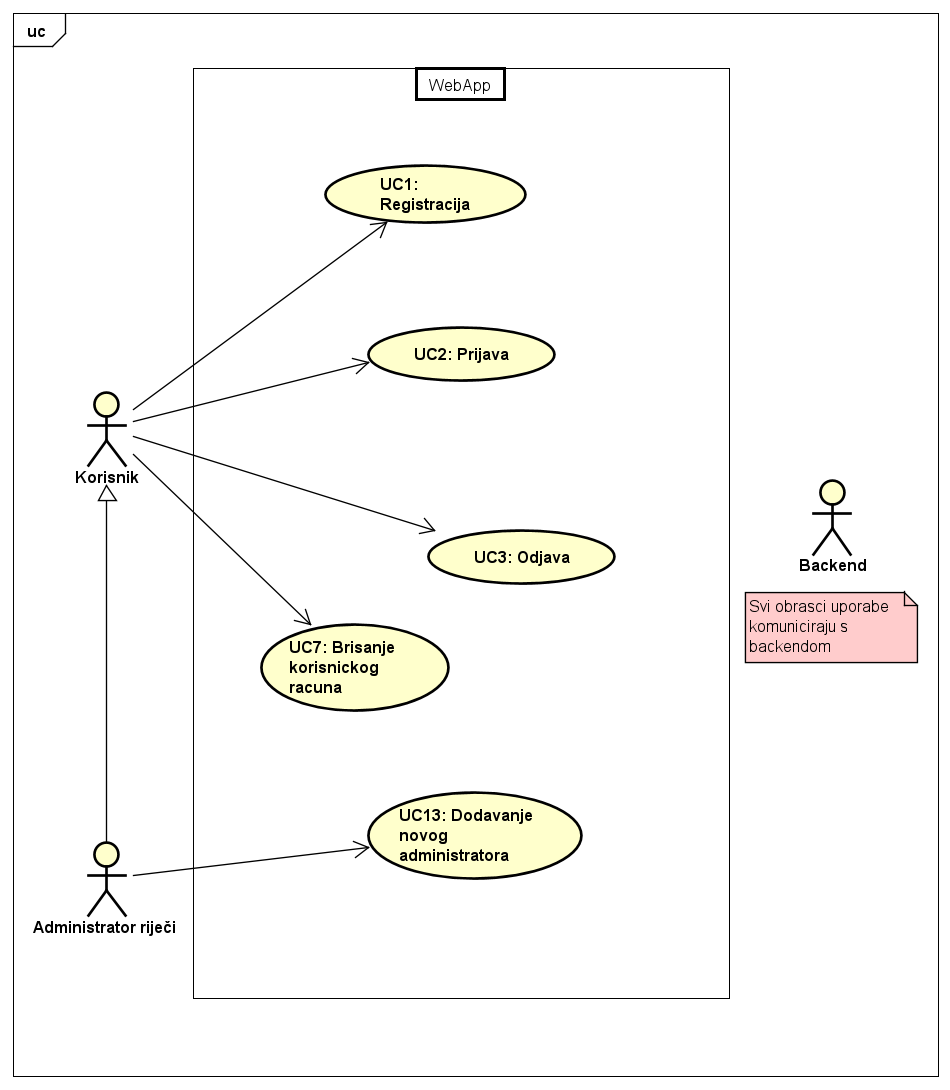
\includegraphics[width=\textwidth]{slike/UseCaseDiagram0.PNG}
						\caption{Dijagram obrazaca uporabe, funkcionalnosti korisnika i administratora riječi}
						\label{fig:useCaseDiagram0}
					\end{figure}
					
					\begin{figure}[H]
						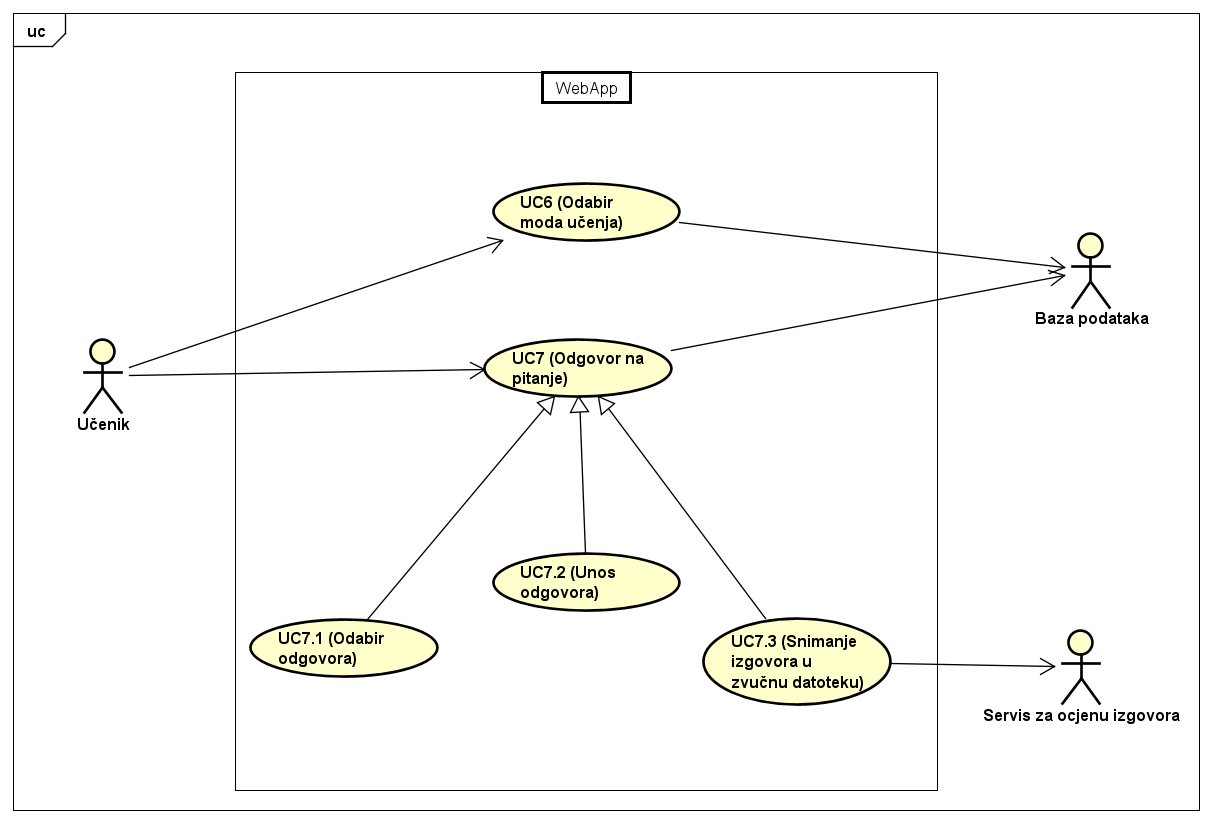
\includegraphics[width=\textwidth]{slike/UseCaseDiagram1.PNG}
						\caption{Dijagram obrazaca uporabe, funkcionalnosti korisnika}
						\label{fig:useCaseDiagram1}
					\end{figure}
					
					\begin{figure}[H]
						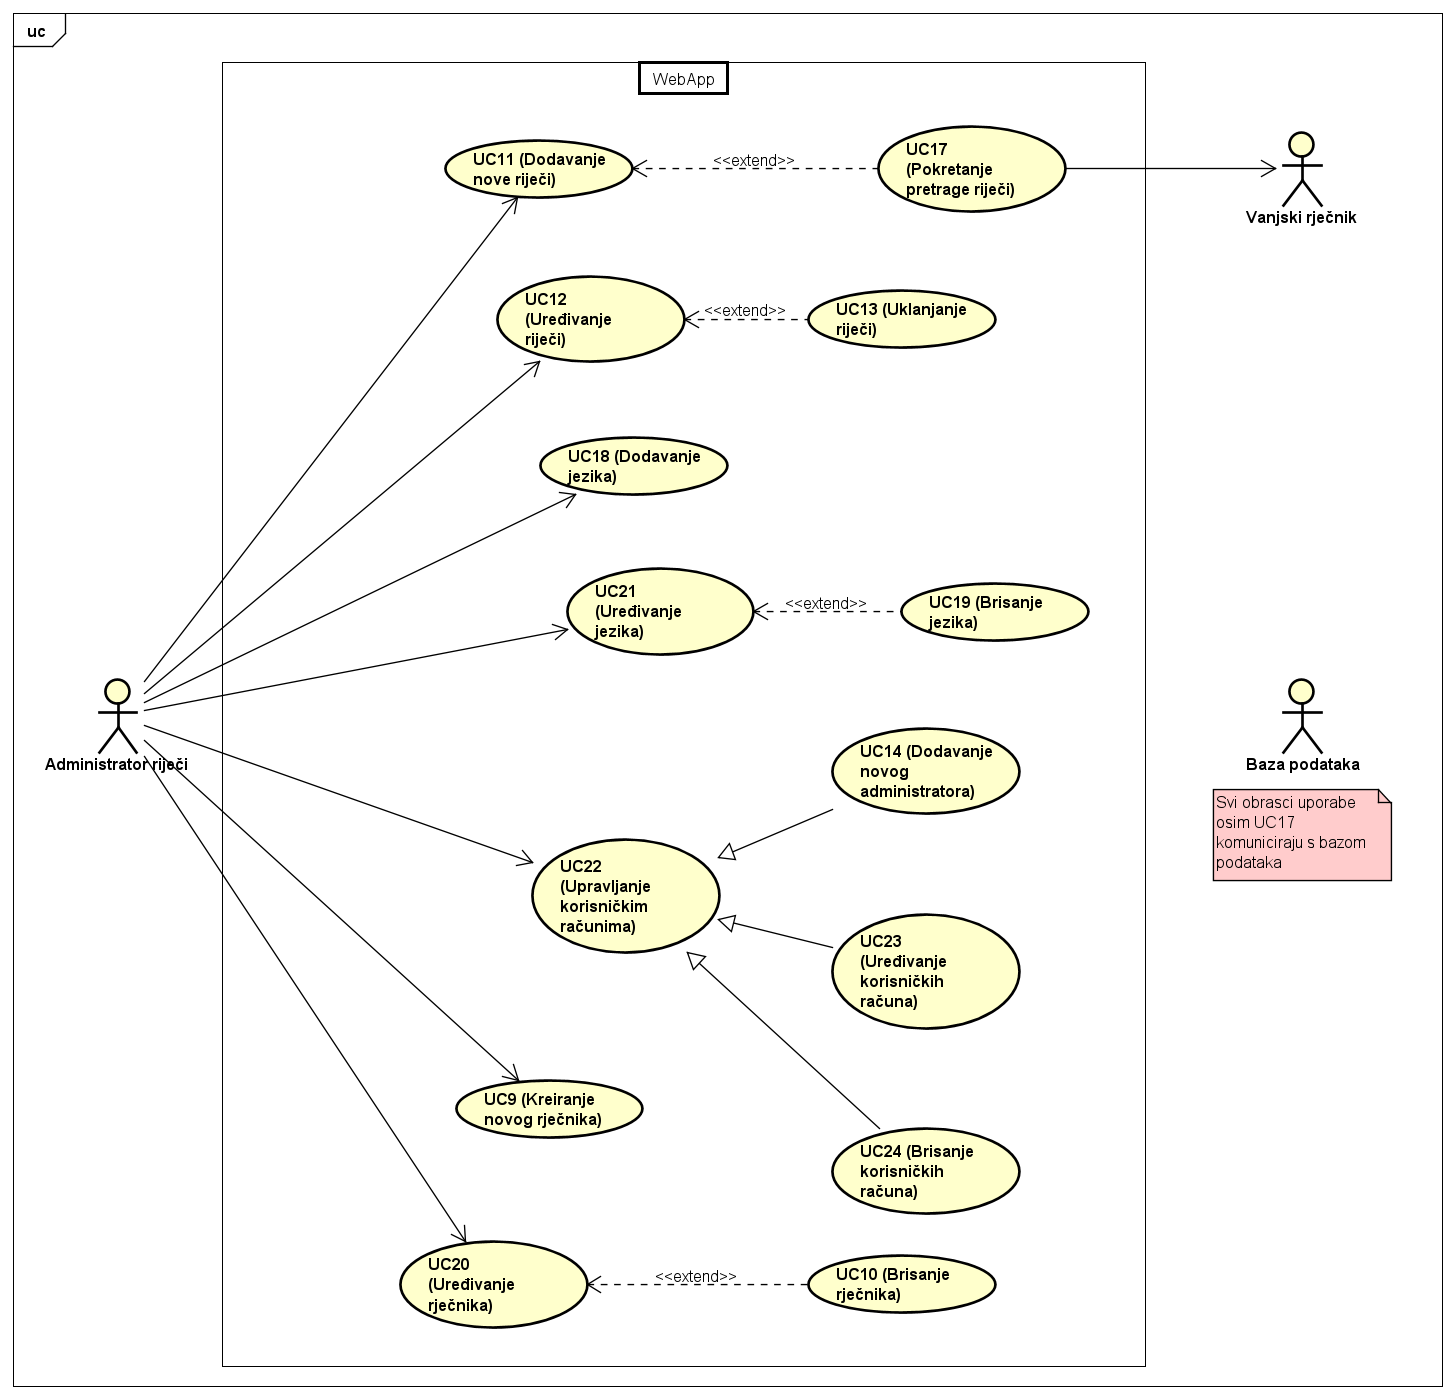
\includegraphics[width=\textwidth]{slike/UseCaseDiagram2.PNG}
						\caption{Dijagram obrazaca uporabe, funkcionalnosti administratora riječi}
						\label{fig:useCaseDiagram2}
					\end{figure} \newpage
				
			\subsection{Sekvencijski dijagrami}
				
%				\textbf{\textit{dio 1. revizije}}\\
%				
%				\textit{Nacrtati sekvencijske dijagrame koji modeliraju najvažnije dijelove sustava (max. 4 dijagrama). Ukoliko postoji nedoumica oko odabira, razjasniti s asistentom. Uz svaki dijagram napisati detaljni opis dijagrama.}
%				\eject
				
				\textbf{Obrazac uporabe UC1- Registracija}\\
				Korisnik odabire opciju „Registracija“. Sustav prikazuje formu za unos podataka za registraciju. Korisnik unosi potrebne podatke i potvrđuje registraciju.. Ako korisnik odustane od registracije, sustav vraća korisnika na početnu stranicu. Ako je korisnik unio mail adresu koja se već koristi u sustavu, sustav vraća obavijest o već registriranoj mail adresi. Ako mail adresa ne postoji u bazi podataka, sustav na navedenu mail adresu šalje mail s inicijalnom lozinkom.\newpage

				\begin{figure}[H]
					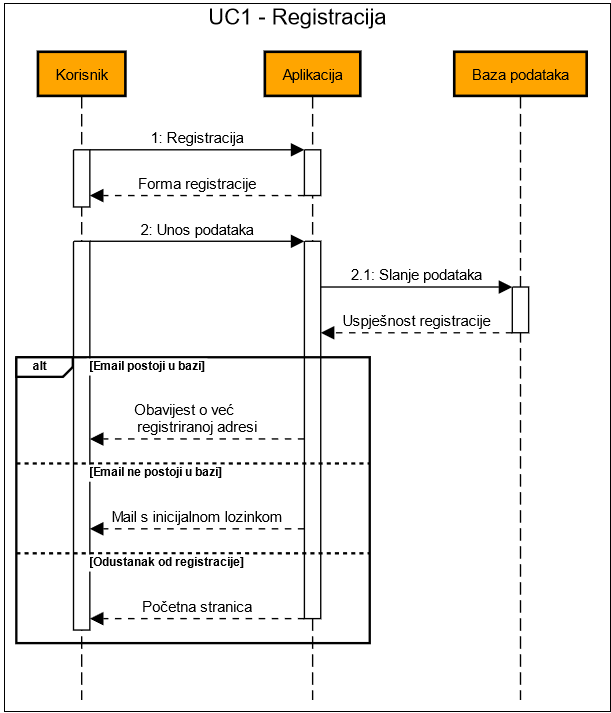
\includegraphics[width=\textwidth]{slike/UC1.PNG}
					\caption{Sekvencijski dijagram za UC1}
					\label{fig:sekv1}
				\end{figure} \newpage
				
				
				\noindent\textbf{Obrazac uporabe UC2 - Prijava}\\
				Korisnik odabire opciju „Prijava“. Sustav prikazuje formu za unos podataka za prijavu. Korisnik unosi potrebne podatke i potvrđuje prijavu. Sustav provjerava ispravnost podataka. Ako su podatci neispravni, sustav šalje obavijest o krivo unesenim podatcima, a korisnik mora ispraviti podatke i ponovno potvrditi prijavu sve dok ne budu uneseni ispravni podatci. Ako se korisnik po prvi puta prijavljuje u sustav, sustav mu prikazuje formu za promjenu inicijalne lozinke. Korisnik unosi novu lozinku, a sustav ju sprema u bazu podataka. Nakon prijave u sustav, sustav šalje korisnika na stranicu s ponuđenim jezicima.
				
				
				\begin{figure}[H]
					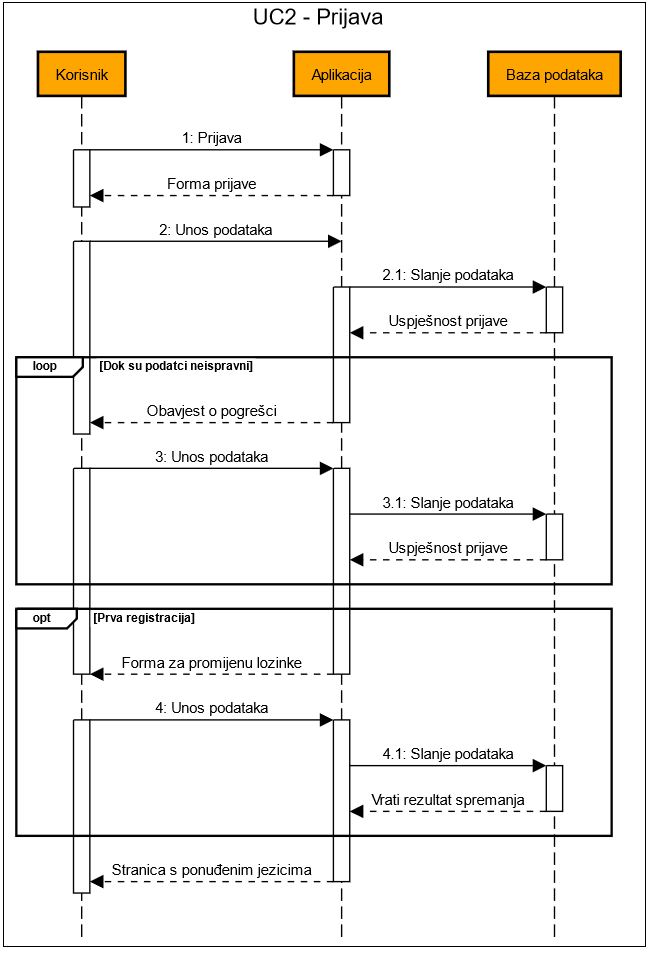
\includegraphics[width=\textwidth]{slike/UC2.PNG}
					\caption{Sekvencijski dijagram za UC2}
					\label{fig:sekv2}
				\end{figure} \newpage
								
				
				
				\noindent\textbf{Obrasci uporabe UC4, UC5 i UC6 - Odabir jezika, Odabir rječnika i moda učenja, Odgovor na pitanje}\\
				Korisnik odabire željeni jezik. Sustav iz baze podataka dohvaća rječnike koji su vezani za odabrani jezik te ih prikazuje korisniku. Korisnik odabire željeni rječnik. Sustav iz baze podataka dohvaća modove učenja te ih prikazuje korisniku. Korisnik odabire mod učenja. Sustav iz baze podataka dohvaća pitanje te prikazuje stranicu s pitanjem. Korisnik odgovara na pitanje te ako je odgovor točan, sustav u bazi podataka odgovoreno pitanje stavlja u iduću posudu. Ako je odgovor netočan, sustav u bazi podataka odgovoreno pitanje stavlja u prvu posudu. Korisnik odabire opciju „Sljedeće pitanje“. Sustav dohvaća novo pitanje iz baze podataka. Ako korisnik odustane od kviza, sustav ga vraća na stranicu s prikazom rječnika.
				
				\begin{figure}[H]
					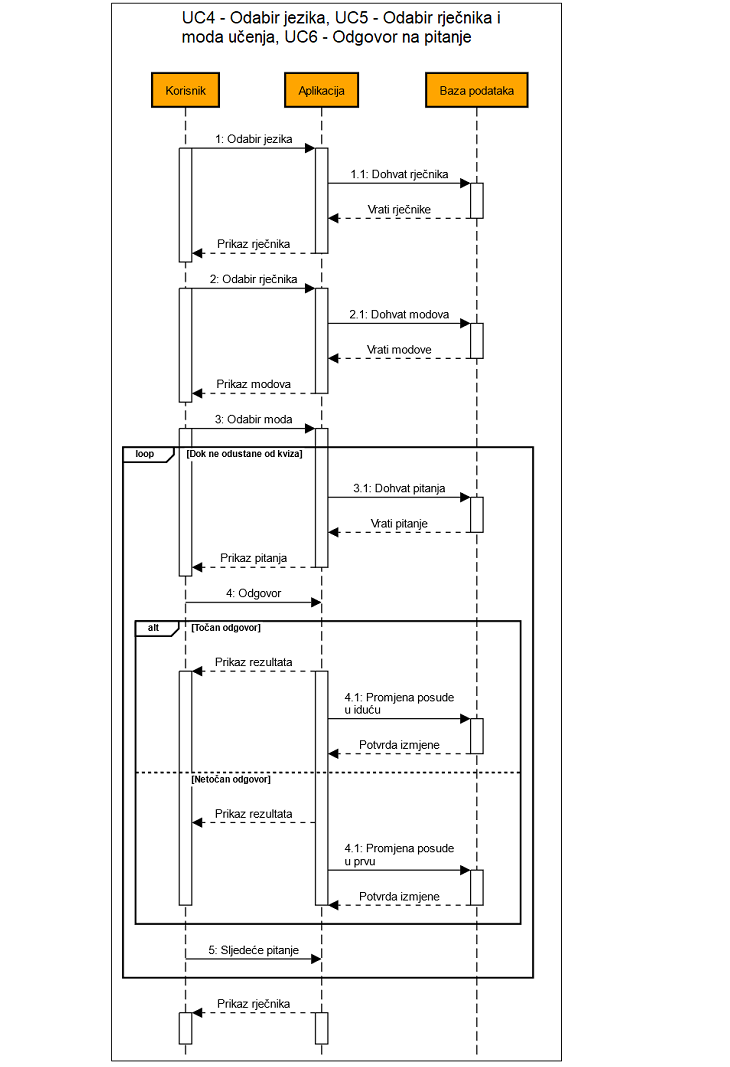
\includegraphics[width=\textwidth]{slike/UC4,UC5,UC6.PNG}
					\caption{Sekvencijski dijagram za UC4, UC5, UC6}
					\label{fig:sekv3}
				\end{figure} \newpage
				
				
				\noindent\textbf{Obrasci uporabe UC8 i UC10 - Kreiranje novog rječnika i Dodavanje nove riječi}\\
				Administrator odabire opciju „Kreiraj novi rječnik“. Sustav prikazuje formu za unos podataka novog rječnika. Administrator upisuje potrebne podatke. Ako su uneseni podatci neispravni, sustav prikazuje obavijest o neispravno unesenim podatcima, a administrator mora ispraviti unesene podatke. Kada su podatci ispravno uneseni, sustav podatke sprema u bazu podataka, a administratoru prikazuje početnu stranicu. Administrator odabire opciju „Dodaj novu riječ“. Sustav prikazuje formu za unos nove riječi. Nakon što administrator unese dio željene riječi, sustav pomoću vanjskih rječnika administratoru dojavljuje savjete s informacijama za unos riječi. Administrator odabire ponuđene riječi, upisuje potrebne podatke te odabire opciju „Spremi“. Sustav novu riječ sprema u bazu podataka, a administratora vraća na početnu stranicu.
				
				\begin{figure}[H]
					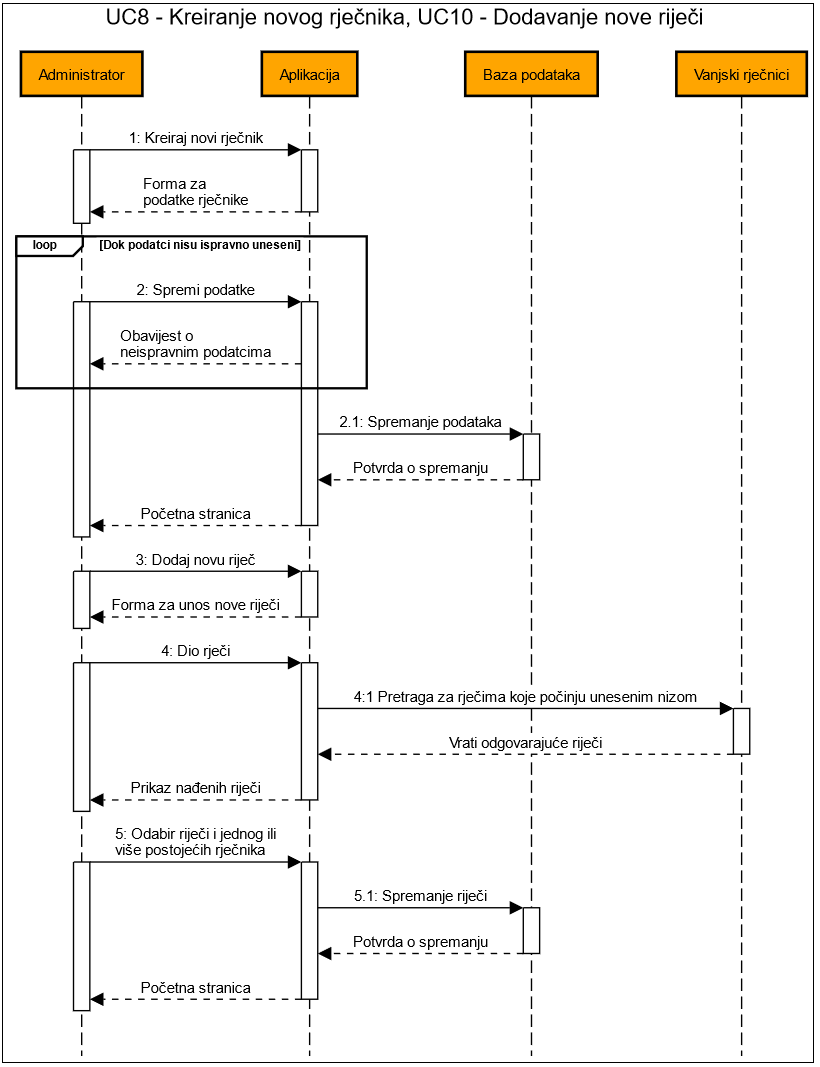
\includegraphics[width=\textwidth]{slike/UC8,UC10.PNG}
					\caption{Sekvencijski dijagram za UC8, UC10}
					\label{fig:sekv4}
				\end{figure} \newpage
	
		\section{Ostali zahtjevi}
		
			\begin{packed_enum}
				
				\item Sustav treba podržavati hrvatski jezik
				\item Sustav treba ostvariti kao web-aplikaciju
				\item Sustav treba koristiti vanjski API za dohvaćanje prijedloga riječi
				\item Sustavu se pristupa uz korištenje protokola HTTPS
				\item Sustav treba ostvariti pomoću objektno orijentiranog jezika
				\item Sve lozinke u sustavu trebaju biti kriptirane radi osiguravanja sigurnosti korisničkih računa
				\item Sustav treba ostvariti tako da bude jednostavan i intuitivan za korištenje
				\item Sustav treba moći pružati uslugu za više korisnika istovremeno
				
			\end{packed_enum}
		
%			\textbf{\textit{dio 1. revizije}}\\
%		 
%			 \textit{Nefunkcionalni zahtjevi i zahtjevi domene primjene dopunjuju funkcionalne zahtjeve. Oni opisuju \textbf{kako se sustav treba ponašati} i koja \textbf{ograničenja} treba poštivati (performanse, korisničko iskustvo, pouzdanost, standardi kvalitete, sigurnost...). Primjeri takvih zahtjeva u Vašem projektu mogu biti: podržani jezici korisničkog sučelja, vrijeme odziva, najveći mogući podržani broj korisnika, podržane web/mobilne platforme, razina zaštite (protokoli komunikacije, kriptiranje...)... Svaki takav zahtjev potrebno je navesti u jednoj ili dvije rečenice.}
			 
			 
			 
	